\subsection{Amplitudenmodulation (AM) S. 51}
Bei der Amplitudenmodulation formt das Nachrichtensignal die Amplitude des Trägersignals (perriodisches Hilfssignal).

\vspace{.1cm}
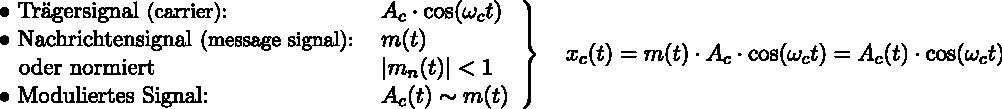
\includegraphics{chapters/06_amplitudenmodulation/figures/AMbasic.pdf}

\vspace{.1cm}
$\rightarrow$ \textbf{Euler}:\hspace{.1cm} \efbox[linecolor=red]{$
		\sin(t) = \frac{1}{2j}\cdot (e^{jt} - e^{.jt}) \qquad
		\cos(t) = \frac{1}{2}\cdot (e^{jt} + e^{.jt})$}

\subsubsection{Frequenzmischer, Frequenzmultiplex S. 46}
Ein \textbf{Frequenzmischer} multipliziert $m_n(t)$ mit einem Träger $\cos(\omega_ct)$ 
oder $\sin(\omega_ct)$ und halbiert; die Bandbreite verdoppelt sich ($B = 2B_m$).

\begin{minipage}{0.6\columnwidth}
	\efbox[linecolor=red]{$A_c \cdot m_n(t) \cdot \cos(\omega_c t)\, \laplace \,\frac{A_c}{2} \cdot \left( M_n(\omega - \omega_c) + M_n(\omega + \omega_c) \right)$}
	\medbreak
	\efbox[linecolor=red]{$A_c \cdot m_n(t) \cdot \sin(\omega_c t)\, \laplace \,\frac{A_c}{2} \cdot \left( -j \cdot M_n(\omega - \omega_c) + j \cdot M_n(\omega + \omega_c) \right)$}
\end{minipage}
\begin{minipage}{0.25\columnwidth}
	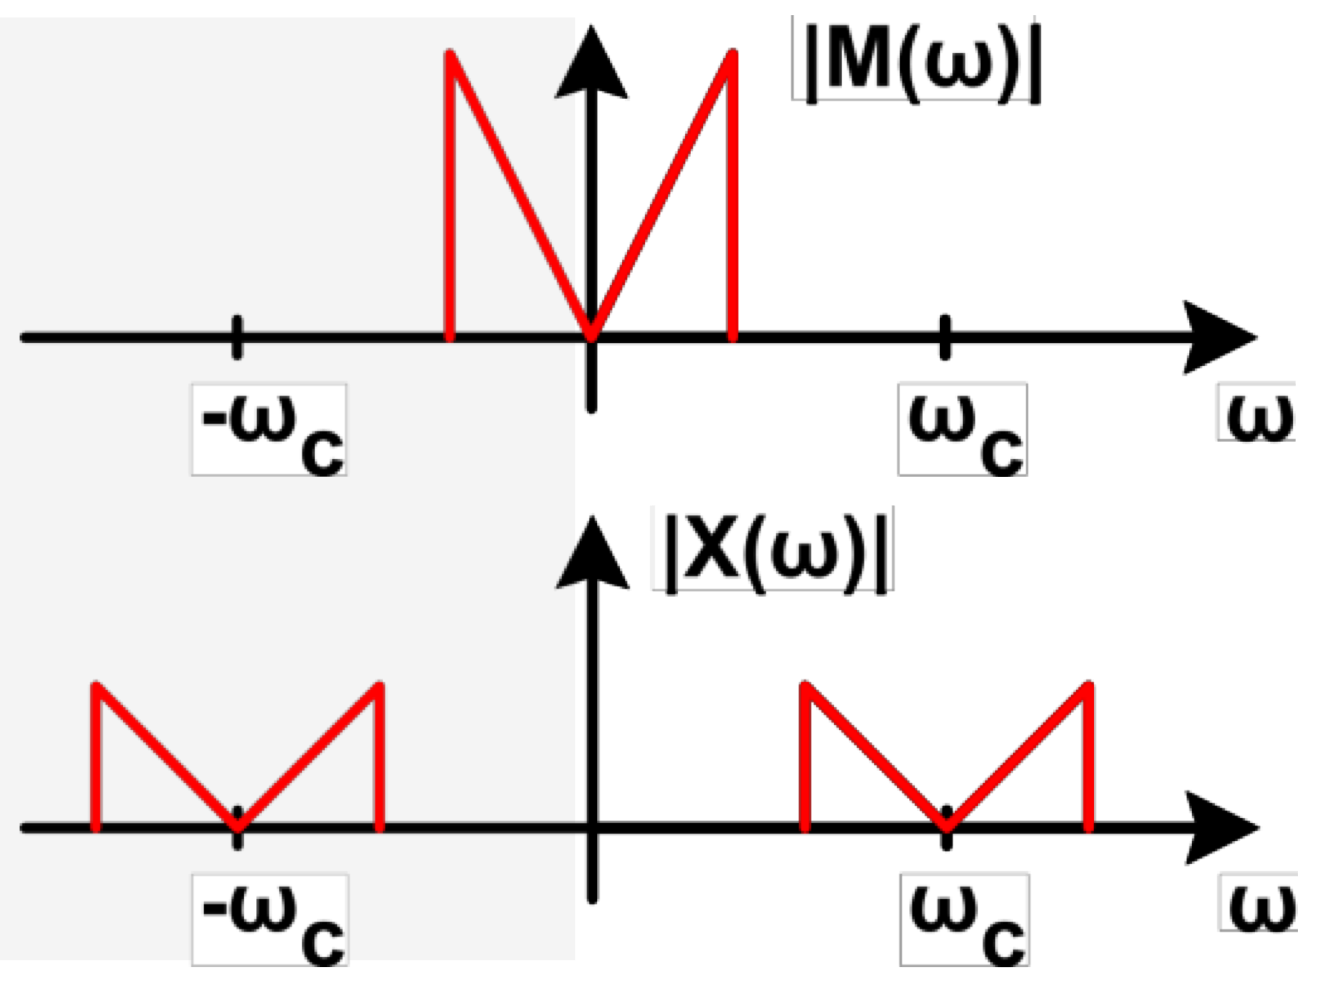
\includegraphics[width=\linewidth]{chapters/06_amplitudenmodulation/figures/frequenzmischer.png}
\end{minipage}

\textbf{Frequenzmultiplex (FDM):} Mehrere Signale werden mit \emph{verschiedenen} 
Trägern $\omega_{c,i}$ in getrennte Frequenzbänder geschoben und gleichzeitig über einen Kanal übertragen. 
Bedingung: Bänder überlappen nicht, d.h. $|\omega_{c,i+1}-\omega_{c,i}| \geq 2\pi 
\cdot 2B_m$.



\subsubsection{Gewöhnliche Amplitudenmodulation S. 51}
Bei der gewöhnlichen AM wird das Nachrichtensignal $m(t)$ mit einem DC offset angehoben um einen Nulldurchgang von $m(t)$ zu verhindern:\hspace{0.01cm} \vspace{.05cm} \efbox[linecolor=red]{$x_{AM}(t) = A_c \cdot (1+\mu \cdot m_n(t)) \cdot cos(\omega_c t)$ \;\; mit $|m(t)| \leq 1$ und Modulationsgrad $\mu$} \\
\textbf{Aufgrund des DC-Anteils ist die gewöhnliche AM nicht linear und nicht zeitinvariant!}

\paragraph{Modulation}
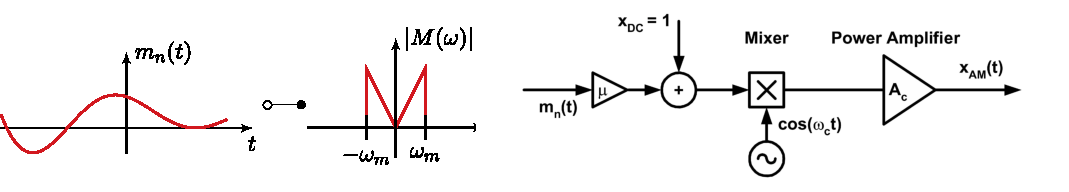
\includegraphics{chapters/06_amplitudenmodulation/figures/AM_grafik.pdf}

\boxedeq{\begin{split}
		x_{_{AM}}(t) = (1 + \mu \cdot m_n(t)) \cdot A_C \cdot  \cos(\omega_c t)
		\; \;\;\; \laplace \;\;\; \; X_{AM}(\omega) = \frac{\mu A_c}{2}  (M(\omega - \omega_c) + 
		M(\omega + \omega_c)) \\ + \pi A_c [\delta (\omega - \omega_c) + 
		\delta (\omega + \omega_c)] \end{split}}

\begin{table}[H]
	\begin{tabularx}{\linewidth}{X X X}
		\begin{minipage}{\linewidth}
		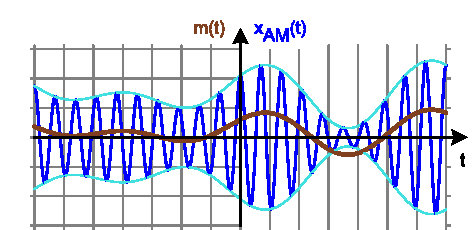
\includegraphics[width=\linewidth]{chapters/06_amplitudenmodulation/figures/abbildung5_10.pdf}
		\end{minipage}
		&
		\begin{minipage}{\linewidth}
		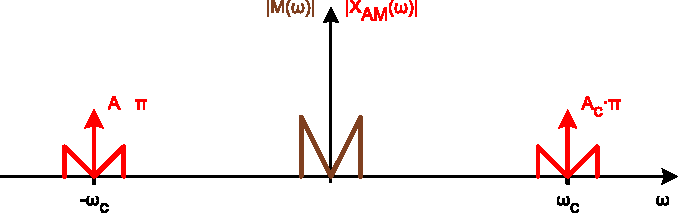
\includegraphics[width=\linewidth]{chapters/06_amplitudenmodulation/figures/abbildung5_12.pdf}
		\end{minipage}
		&
		\begin{minipage}{1.05\linewidth}
			\textbf{DC-Anteil:} bewirkt, dass Carrier im Frequenzbereich nicht verschwindet \\
			\textbf{Modulationsindex $\mu$ :} $0 < \mu < 1$ \\
			$\mu > 1$ $\rightarrow$ Übermodulation \\
			 \efbox[linecolor=red]{$\mu = \frac{\max|x_{AM}|-min|x_{AM}|}{\max|x_{AM}|+min|x_{AM}|} $}
		\end{minipage}
	\end{tabularx}
\end{table}

\begin{tabular}{m{10cm} m{5cm}}
\paragraph{Demodulation}\mbox{ }
		\vspace{.2cm}
	
	\begin{list}{$\bullet$}{\setlength{\itemsep}{0cm} \setlength{\parsep}{0cm} 	\setlength{\topsep}{0cm}} 
		\item Hüllkurvendetektor (Envelope Detector) S.51
		\item Kohärente Produktdemodulation (siehe DSB-SC)
	\end{list}
\vspace{.5cm}
	\textbf{Bedingungen für Envelop-Demodulation}
	\vspace{.2cm}
	
	\begin{minipage}{\linewidth}
	\begin{list}{$\bullet$}{\setlength{\itemsep}{0cm} \setlength{\parsep}{0cm} 	\setlength{\topsep}{0cm}} 
		\item Umhüllende darf \textbf{nicht unter Null} fallen
		\item Modulationsindex $0 < \mu < 1$, bei Übermodulation fällt Umhüllende unter Null
		\item optimale Zeitkonstante des Hüllkurvendetektors \\
		$B_m < \frac{1}{RC} << f_c $ mit $B_m$: Bandbreite von $m(t)$
	\end{list}
	\end{minipage}
	
	&
	\begin{minipage}{0.4\linewidth}
		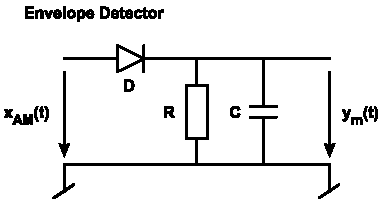
\includegraphics{chapters/06_amplitudenmodulation/figures/abbildung5_9.pdf}
		
		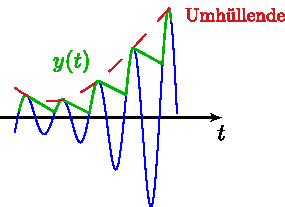
\includegraphics{chapters/06_amplitudenmodulation/figures/envelope_graph.pdf}
	\end{minipage}

\end{tabular}

\newpage
\paragraph{Äquivalente Basisbanddarstellung der gewöhnlichen AM S. 53}
\emph{Idea:} si sostituisce la portante reale ad alta frequenza con un \textbf{fasore complesso} $x_{eq}(t)$ che contiene ampiezza e fase $\rightarrow$ si calcola solo col segnale lento in banda base.

\begin{minipage}[t]{.52\textwidth}
	$x_{AM}(t) = A_c(1+\mu m_n)\cdot\tfrac{1}{2}\left(e^{+j\omega_c t}+e^{-j\omega_c t}\right)$\\[.05cm]
	\emph{Tre semplificazioni:}
	\begin{enumerate}\setlength{\itemsep}{0pt}\setlength{\parsep}{0pt}\setlength{\topsep}{0pt}
		\item \textbf{Togli il fasore a $-\omega_c$}: è sempre il coniugato del primo, nessuna info in più ($v+v^*=\Re\{2v\}$).
		\item \textbf{Non scrivere $\Re\{\cdot\}$}: sottinteso, si prende alla fine.
		\item \textbf{Non scrivere $e^{+j\omega_c t}$}: rotazione nota e uguale per tutti, non cambia l'inviluppo.
	\end{enumerate}
\end{minipage}\hfill
\begin{minipage}[t]{.45\textwidth}
	\efbox[linecolor=red]{$x(t) = \Re\{x_{eq}(t)\, e^{j\omega_c t}\}$, \; $x_{eq} = I + jQ = |x_{eq}|\, e^{j\varphi}$}\\[.05cm]
	$\Rightarrow x(t) = I\cos(\omega_c t) - Q\sin(\omega_c t)$\\
	$I$: in fase (asse orizz.), $Q$: in quadratura (asse vert.)\\
	$|x_{eq}|$ = inviluppo, $\arg x_{eq}$ = fase\\[.05cm]
	\textbf{Träger $\rightarrow$ Zeiger:} $\cos(\omega_c t+\varphi)\rightarrow e^{j\varphi}$\\
	$\cos \rightarrow 1,\ \sin \rightarrow -j,\ -\cos \rightarrow -1,\ -\sin \rightarrow +j$
\end{minipage}

\vspace{.1cm}
Si disegna la \textbf{Ortskurve} di $x_{eq}$ (tutti i valori assunti, senza l'andamento nel tempo). AM: il punto si muove solo su una \textbf{retta per l'origine} (fase fissa, cambia solo la lunghezza).

% Ortskurve: #1 Winkel [deg], #2 r_min, #3 r_max, #4/#5 Beschriftung min/max, #6/#7 Anker min/max
\newcommand{\eqbaseplot}[7]{%
	\begin{tikzpicture}[scale=.6,>=stealth,font=\scriptsize]
		\draw[->] (-2.3,0) -- (2.9,0) node[above left,inner sep=1pt]{$I=\Re$};
		\draw[->] (0,-2.3) -- (0,2.7) node[below right]{$Q=\Im$};
		\draw[gray!70] (0,0) circle (1);
		\foreach \x/\l/\a in {1/1/south west,-1/-1/south east}{\draw (\x,-.07)--(\x,.07); \node[anchor=\a,inner sep=1pt] at (\x,0) {$\l$};}
		\foreach \y/\l/\a in {1/j/south east,-1/-j/north east}{\draw (-.07,\y)--(.07,\y); \node[anchor=\a,inner sep=1pt] at (0,\y) {$\l$};}
		\draw[gray!60,dashed] (0,0) -- (#1:#2);
		\draw[red,line width=1.6pt] (#1:#2) -- (#1:#3);
		\fill[red] (#1:#2) circle (1.6pt) node[anchor=#6,text=red,inner sep=2pt]{#4};
		\fill[red] (#1:#3) circle (1.6pt) node[anchor=#7,text=red,inner sep=2pt]{#5};
	\end{tikzpicture}}

\noindent\begin{tabularx}{\textwidth}{>{\centering\arraybackslash}X >{\centering\arraybackslash}X >{\centering\arraybackslash}X >{\centering\arraybackslash}X}
	\textbf{Cosinus}, $\mu=\qty{25}{\%}$ & \textbf{Sinus}, $\mu=\qty{50}{\%}$ & \textbf{Cos $+\frac{\pi}{4}$}, $\mu=\qty{100}{\%}$ & \textbf{Übermod.}, $\mu=\qty{150}{\%}$ \\
	\eqbaseplot{0}{0.75}{1.25}{$0.75$}{$1.25$}{south east}{north west} &
	\eqbaseplot{-90}{0.5}{1.5}{$-0.5j$}{$-1.5j$}{west}{west} &
	\eqbaseplot{45}{0}{2}{$0$}{$\sqrt2(1+j)$}{north west}{north west} &
	\eqbaseplot{0}{-0.5}{2.5}{$-0.5$}{$2.5$}{north}{north east} \\
	\efbox[linecolor=red]{$x_{eq}=A_c(1+\mu m_n)$} &
	\efbox[linecolor=red]{$x_{eq}=-j A_c(1+\mu m_n)$} &
	\efbox[linecolor=red]{$x_{eq}=\tfrac{1+j}{\sqrt2}A_c(1+\mu m_n)$} &
	$x_{eq}<0$: salto di fase \ang{180} \\[.25cm]
	\footnotesize $A_c=1$ &
	\footnotesize $\sin(\omega_c t)=\Re\{-j\,e^{j\omega_c t}\}$ &
	\footnotesize $e^{j\pi/4}=\tfrac{1+j}{\sqrt2}$, $|x_{eq}|\le 2$ &
	\footnotesize passa per $0$ $\rightarrow$ Hüllkurvendet. non funziona
\end{tabularx}

\vspace{.1cm}
\textbf{Merke:} AM $\rightarrow$ segmento (cambia solo $|x_{eq}|$), PM/FM $\rightarrow$ arco di cerchio (cambia solo $\varphi$), QAM $\rightarrow$ tutto il piano ($I$, $Q$ indipendenti).

\paragraph{Leistungseffizienz der gewöhnlichen AM S. 56}
Unter der Effizienz $\eta$ der gewöhnlichen AM versteht man das Verhältnis von Signalleistung $P_s$ der \textbf{beiden Seitenbänder} zur Gesamtleistung $P_t$ des AM-Signals.
\begin{equation*}
	P_c = \frac{A_c^2}{2} \;\; \text{und} \;\; P_t = \frac{A_c^2}{2} + \frac{A_c^2 \mu^2P_m}{2} \rightarrow \eta = \frac{P_s}{P_t} = \frac{P_t - P_c}{P_t} = \frac{\mu^2P_m}{1+\mu^2P_m} = \frac{(\frac{\mu}{C})^2}{1+(\frac{\mu}{C})^2} = \frac{\mu^2 \cdot m^2_{rms}}{1+\mu^2 \cdot m^2_{rms}}
\end{equation*}
Die maximal mögliche Effizienz ($\mu = \qty{100}{\%}$) beträgt \qty{33}{\%}. Bei $\mu = \qty{50}{\%}$ sind noch \qty{11.1}{\%} möglich.

\subsubsection{DSB-SC - Zweiseitenbandamplitudenmodulation ohne Träger S. 58}
Double-Sideband Suppressed-Carrier Modulation
\paragraph{Modulation}

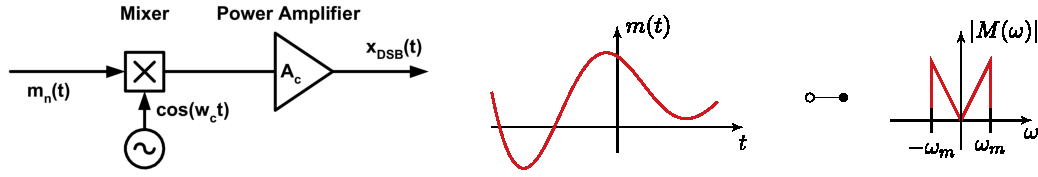
\includegraphics{chapters/06_amplitudenmodulation/figures/DCBmodulation_grafik.pdf}
\begin{table}[H]
	\begin{tabularx}{\linewidth}{X X X}
		\begin{minipage}{\linewidth}
			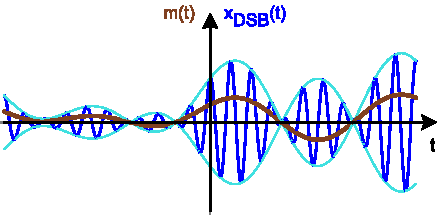
\includegraphics[width=\linewidth]{chapters/06_amplitudenmodulation/figures/abbildung5_17.pdf}
		\end{minipage}
		&
		\begin{minipage}{\linewidth}
			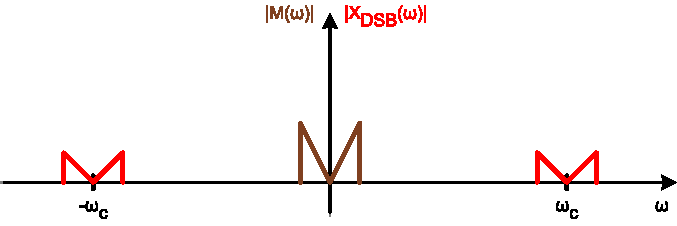
\includegraphics[width=\linewidth]{chapters/06_amplitudenmodulation/figures/abbildung5_18.pdf}
		\end{minipage}
		&
		\begin{minipage}{1\linewidth}
			\textbf{Bandbreite:} \\$X(\omega) = 2 \cdot \text{ Bandbreite } M(\omega)$ \\
			\textbf{Amplitude:} \\$1/2 \text{ Amplitude } M(\omega)$\\
			(wenn $A_c = 1$)
		\end{minipage}
	\end{tabularx}
\end{table}
\textbf{DSB-SC ist linear, aber nicht zeitinvariant!} Trotzdem wird AM oft als lineare Modulation bezeichnet. Weil bei DSB-C und gewöhnlicher AM das Spektrum nur verschoben wird.

\paragraph{Demodulation S. 59}
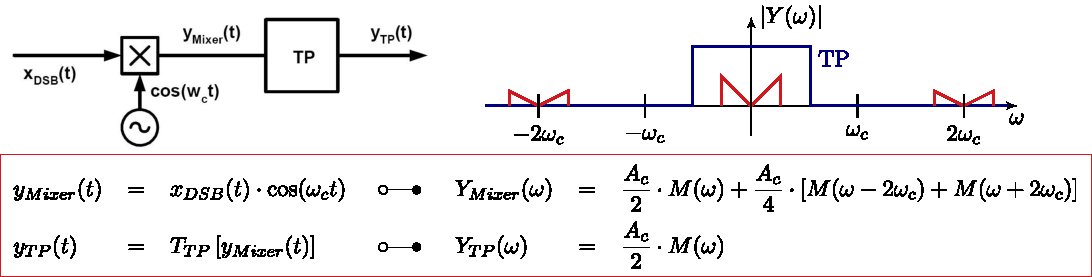
\includegraphics{chapters/06_amplitudenmodulation/figures/DSB_SC_demodulation.pdf}

Das DSB-Signal wird mit einem sogenannten \textbf{synchronen Demodulator} oder \textbf{kohärenten Demodulator} zurückgewonnen. Weicht die \textbf{Frequenz oder die Phase} des demodulierten, lokalen Trägers von dem, des ursprünglichen Trägers ab, so ergibt sich eine \textbf{Abschwächung im demodulierten Signal}.

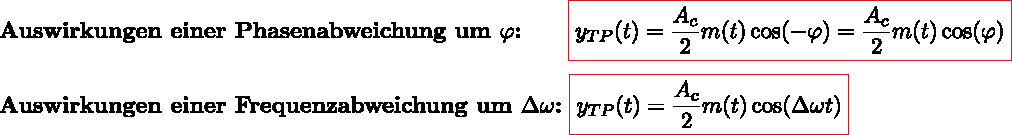
\includegraphics{chapters/06_amplitudenmodulation/figures/demod_abweichung.pdf}

\subsubsection{Einseitenbandamplitudenmodulation (SSB) S. 60}
Bei der SSB Modulation wird \textbf{nur ein Seitenband übertragen}. Die Implementierung gegenüber gewöhnlicher AM und DSB ist komplexer.
\paragraph{Modulation - Filtermethode S. 61}
Mit einem Bandpassfilter kann entweder das USB (upper side band) oder das LSB (lower side band) unterdrückt werden um ein Einseitenband-Signal zu erhalten. Allerdings stellt dies \textbf{hohe Anforderungen an die Flankensteilheit} des Filters.

\paragraph{Modulation - Phasenmethode}
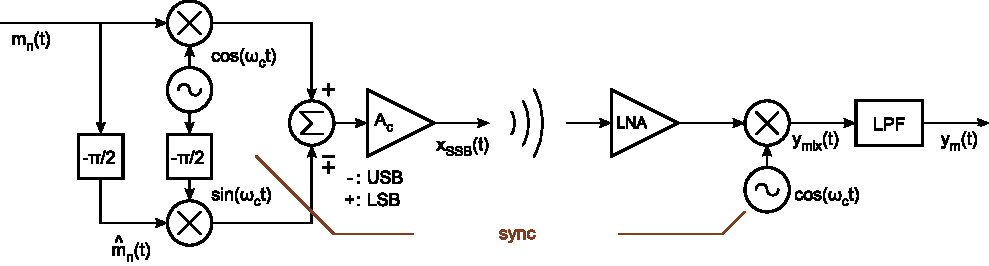
\includegraphics{chapters/06_amplitudenmodulation/figures/abbildung5_23.pdf}
\begin{table}[H]
	\begin{tabularx}{\linewidth}{X X}
		\begin{minipage}{\linewidth}
			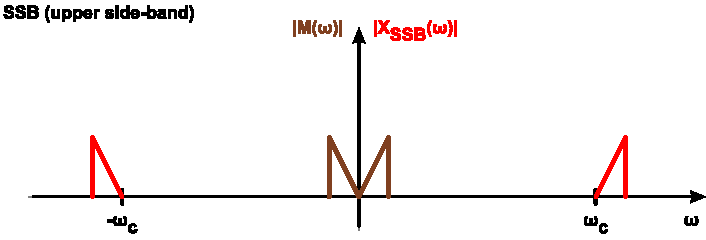
\includegraphics[width=\linewidth]{chapters/06_amplitudenmodulation/figures/abbildung5_22_1.pdf}
		\end{minipage}
	&
	\begin{minipage}{\linewidth}
		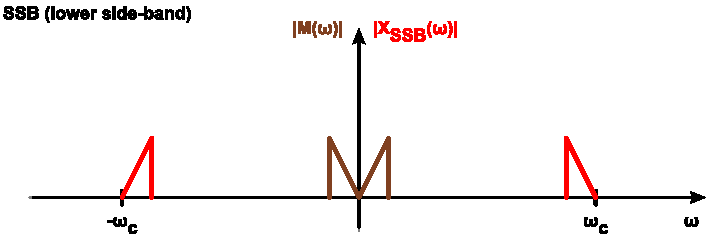
\includegraphics[width=\linewidth]{chapters/06_amplitudenmodulation/figures/abbildung5_22_2.pdf}
	\end{minipage}
	\end{tabularx}
\end{table}
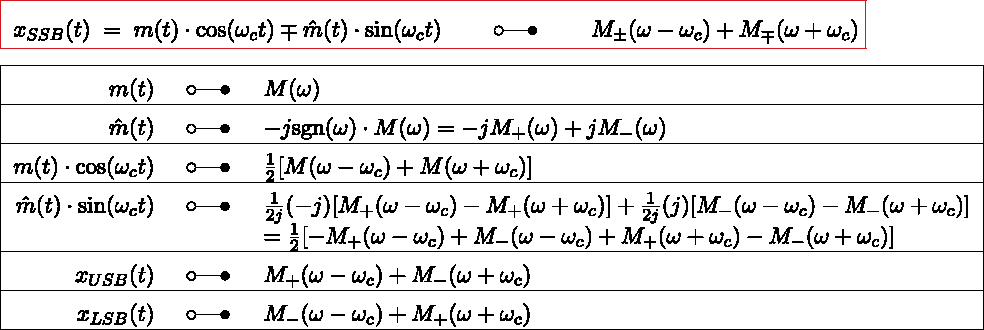
\includegraphics{chapters/06_amplitudenmodulation/figures/SSB_phasenmethode.pdf}

\paragraph{Demodulation S. 63}
\textbf{Kohärente Demodulation ist erforderlich!}

\includegraphics{chapters/06_amplitudenmodulation/figures/SSB_demod.pdf}

\subsubsection{Restseitenband-Amplitudenmodulation (VSB) S. 64}
Siehe auch Folie 23 NaT1\underline{ }3c; Restseitenband-AM ist ein Kompromiss zwischen:
\begin{list}{$\bullet$}{\setlength{\itemsep}{0cm} \setlength{\parsep}{0cm} 	\setlength{\topsep}{0cm}} 
	\item Bandbreiteneffizienz von SSB (1.25 x Bandbreite von SSB)
	\item Einfacher technischer Realisierung von DSB (keine extremen Anforderungen an Filtersteilheit)
\end{list}
\paragraph{Modulation}
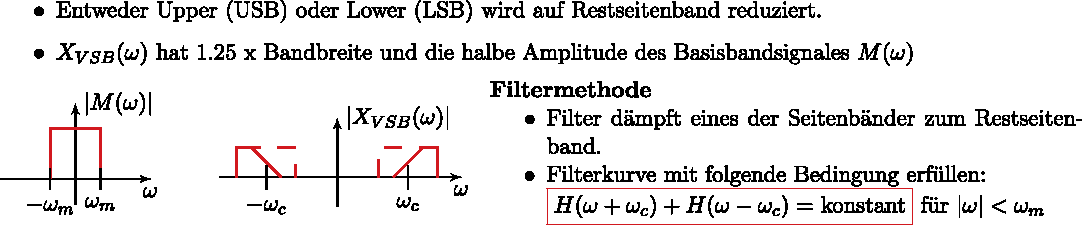
\includegraphics{chapters/06_amplitudenmodulation/figures/VSB_mod.pdf}
\paragraph{Demodulation}
\textbf{Kohärente Demodulation ist erforderlich!}\\
Demodulation erfolgt gleich wie bei SSB-AM

\subsubsection{Quadraturamplitudenmodulation (QAM) S. 64}
Gleichzeitige Übertragung von zwei Basisbandsignalen im gleichen Frequenzband aber mit zwei orthogonalen Trägersignalen $cos(\omega_c t)$ und $sin(\omega_c t)$.\\
Vorteil: ebenso hohe Bandbreiteneffizienz wie SSB-AM \\
Nachteil: technisch aufwändiger als DSB-AM
\paragraph{Modulation und Demodulation S. 65}
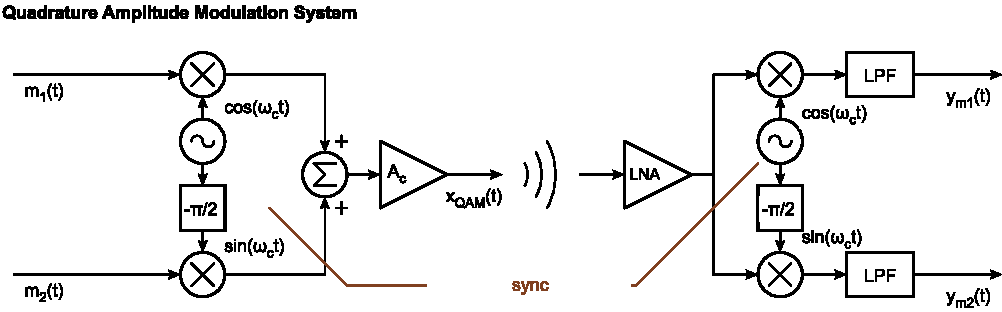
\includegraphics[width=.8\linewidth]{chapters/06_amplitudenmodulation/figures/abbildung5_25.pdf}\\
\efbox[linecolor=red]{$B_{QAM} = 2\cdot max(B_{m1}, B_{m2}) $} $\rightarrow$ gleich wie DSB; Wenn $m_1$ die Hilberttrafo von $m_2$ ist, dann Bandbreite wie SSB $B_{SSB} = B_m$